\documentclass[a4paper,12pt]{article}

% Import the deliverable package from common directory
\usepackage{../common/deliverable}

% Tell LaTeX where to find graphics files
\graphicspath{{../common/logos/}{./figures/}{../}}

\usepackage{xspace}
\usepackage{lipsum}
\usepackage{subcaption}
\usepackage{amsmath}

% Set the deliverable number (without the D prefix, it's added automatically)
\setdeliverableNumber{1.7}

% Begin document
\begin{document}

% Create the title page with the title as argument
\maketitlepage{Improvements to deal.II}

\newpage

% Main Table using the new environment and command
\begin{deliverableTable}
    \tableEntry{Deliverable title}{Improvements to deal.II}
    \tableEntry{Deliverable number}{D1.7}
    \tableEntry{Deliverable version}{[Version number]}
    \tableEntry{Date of delivery}{[Planned date]}
    \tableEntry{Actual date of delivery}{[Actual date]}
    \tableEntry{Nature of deliverable}{[Report/Demonstrator/Website/etc.]}
    \tableEntry{Dissemination level}{[Public/Confidential]}
    \tableEntry{Work Package}{WP[X]}
    \tableEntry{Partner responsible}{[Lead partner acronym]}
\end{deliverableTable}

% Abstract and Keywords Section
\begin{deliverableTable}
    \tableEntry{Abstract}{\lipsum[1][1-5]}
    \tableEntry{Keywords}{Keyword 1; Keyword 2; Keyword 3; Keyword 4; Keyword 5}
\end{deliverableTable}

\newpage

\begin{documentControl}
    \addVersion{0.1}{21/02/2026}{Marco Feder}{Initial draft}
    \addVersion{0.2}{22/02/2026}{Marco Feder}{Polygonal discretization module section}

\end{documentControl}

\subsection*{{Approval Details}}
Approved by: [Name] \\
Approval Date: [Date]

\subsection*{{Distribution List}}
\begin{itemize}
    \item [] - Project Coordinators (PCs)
    \item [] - Work Package Leaders (WPLs)
    \item [] - Steering Committee (SC)
    \item [] - European Commission (EC)
\end{itemize}

\vspace*{2cm}

\disclaimer

\newpage

\tableofcontents % Automatically generated and hyperlinked Table of Contents

\newpage

\section{{Introduction}}



\subsection{{Purpose of the Document}}


\subsection{{Structure of the Document}}
\begin{itemize}
    \item Section \ref{sec:section2}: [Pre-exascale capabilities of deal.II]
    \item Section \ref{sec:section3}: [Pre-exascale modules of deal.II]
    \item Section \ref{sec:section4}: [Polygonal discretization module]
    \item Section \ref{sec:section5}: [Integration of PSCToolkit]
    \item Section \ref{sec:section6}: [Integration of MUMPS]
\end{itemize}

\newpage

\section{{Pre-exascale capabilities of deal.II}}
\label{sec:section2}

\subsection{{[Subsection Title]}}


\newpage

\section{{Pre-exascale modules of deal.II}}
\label{sec:section3}


\newpage

\section{{Polygonal discretization module}}
\label{sec:section4}

The polygonal discretization module described in Work Package 1.5 has undergone exhaustive testing and validation. The new library
associated with this module, \texttt{Polydeal}, is available at \url{https://github.com/fdrmrc/Polydeal}. Some features available in this
module are designed to be integrated into the deal.II library. In order to guarantee maximum compatibility, it is updated to the latest version of deal.II, and it is developed following the same coding style and practices.
A comprehensive test suite is deployed at each new commit on the continuous integration system to guarantee the integrity of the codebase.

\subsection{Geometrically informed multilevel preconditioning}
Large-scale simulations require efficient preconditioners for the iterative solution of the linear systems arising from finite element discretizations, for instance with discontinuous Galerkin (DG) methods. For elliptic problems, geometric multigrid methods are among the most effective preconditioners. However, their application requires the construction of a mesh hierarchy, which can be challenging for fine, unstructured geometries. In such cases, AMG methods are often employed as an alternative. One of the key features of polytopal methods is precisely their very good interplay with DG methodologies (see e.g.,~\cite{polyDG,Antoniettihp}). In particular, the
flexibility of DG methods allows the usage of very general agglomerated grids, i.e.\ grids obtained by merging together several elements of a
finer grid.


By exploiting the efficient agglomeration routine developed in~\cite{FEDER2025113773}, already available in \texttt{Polydeal}, it is possible to construct
a hierarchy of \emph{nested} agglomerated grids, for which intergrid transfer operators among consecutive levels are cheap. This hierarchy naturally enables the construction of multilevel preconditioners for DG discretizations of elliptic problems, leveraging polytopal grids on coarser levels, while keeping the \emph{original} grid unchanged. Coarser operators can be obtained by rediscretization of the partial differential
equation on the agglomerated grids, or by triple Galerkin projection\footnote{This means that coarser operators are recursively obtained by restriction of the finer operators, in an algebraic multigrid sense.}. The latter approach is particularly appealing, since it
allows obtaining coarser operators without the need of rediscretization on agglomerated meshes.

This technique has been successfully applied in~\cite{feder2026agglomeration} to the DG discretization of the monodomain model arising in cardiac electrophysiology. More precisely, we have developed a novel multigrid solver for its DG discretization, exploiting agglomerated
grids on coarser levels. The resulting preconditioner builds coarser operators in an algebraic multigrid fashion, injecting geometric information through the agglomeration routine. In this sense, we
have devised a \emph{geometrically informed} multigrid preconditioner, with the geometric information being injected through the agglomeration routine.

Finally, the linear system of equations associated with the model is solved, at each time-step, with a conjugate-gradient method preconditioned by one V-cycle of our multigrid scheme. The preconditioner has been successfully applied to several test cases, including high-order polynomial degrees, and a realistic 3D ventricular geometry, shown in Figure~\ref{fig:left_ventricle}. Since the
finest level of the multigrid hierarchy consists of an hexahedral grid, we leverage the tensor-product structure of the basis functions and quadrature points in order to exploit state-of-the-art matrix-free operator evaluation techniques developed in~\cite{KronbichlerKormann}, which form a key part of the computational backbone of
the \texttt{deal.II} library.

In Figure~\ref{fig:iterates_3D_monodomain}, we report the number of iterations throughout all the simulation, comparing our agglomerated multigrid preconditioner with the AMG implementation available in the Trilinos ML package. The results are reported
for polynomial degrees $p\!=\!1,2$ for the three-dimensional ventricle mesh. It is evident how
the iteration counts of the AMG preconditioner are always higher than the agglomeration-based multigrid approach. The actual wall-clock
times (in seconds) are reported in Figure~\ref{fig:iteration_times_3D_monodomain}, showing a huge reduction of the time per iteration when using
the agglomeration-based multigrid strategy. A detailed discussion on the costs can be found in~\cite{feder2026agglomeration}.


The obtained results indicate the high effectiveness of the preconditioner in terms of iteration counts and robustness with respect to model parameters. Despite these encouraging results, several research directions remain open to further enhance the efficiency and scalability of the preconditioner. In this sense, integration
within existing AMG frameworks is a promising direction, along with the development of matrix-free implementations of the coarser operators, which would further reduce the
application cost of the preconditioner.




\begin{figure}
    \centering
    \begin{subfigure}{0.30\linewidth}
        \centering
        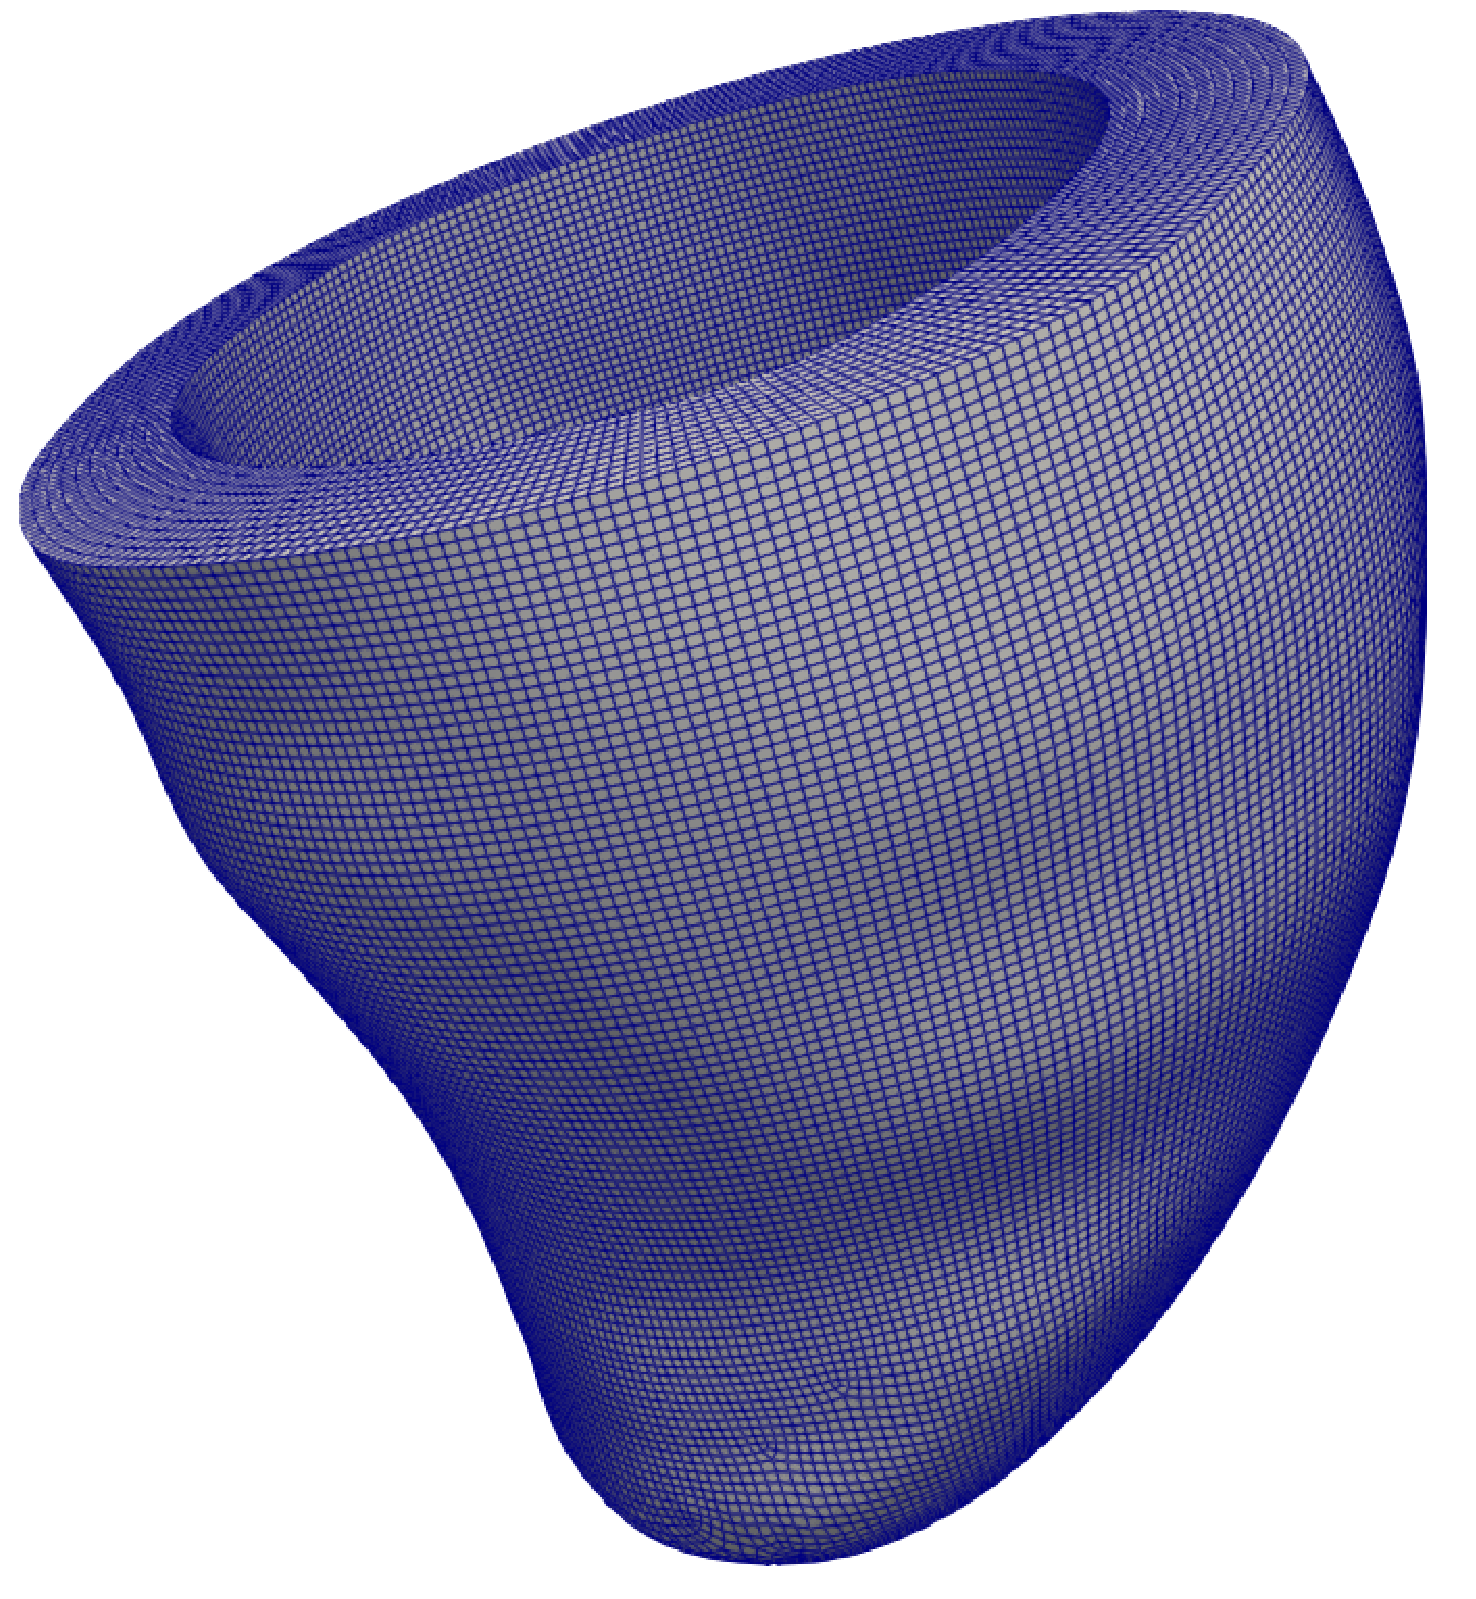
\includegraphics[width=\linewidth]{fig/left_ventricle_view-cropped.pdf}
        \caption{}
        \label{subfig:left_ventricle_mesh}
    \end{subfigure}
    \hspace{4cm}
    \begin{subfigure}{0.30\linewidth}
        \centering
        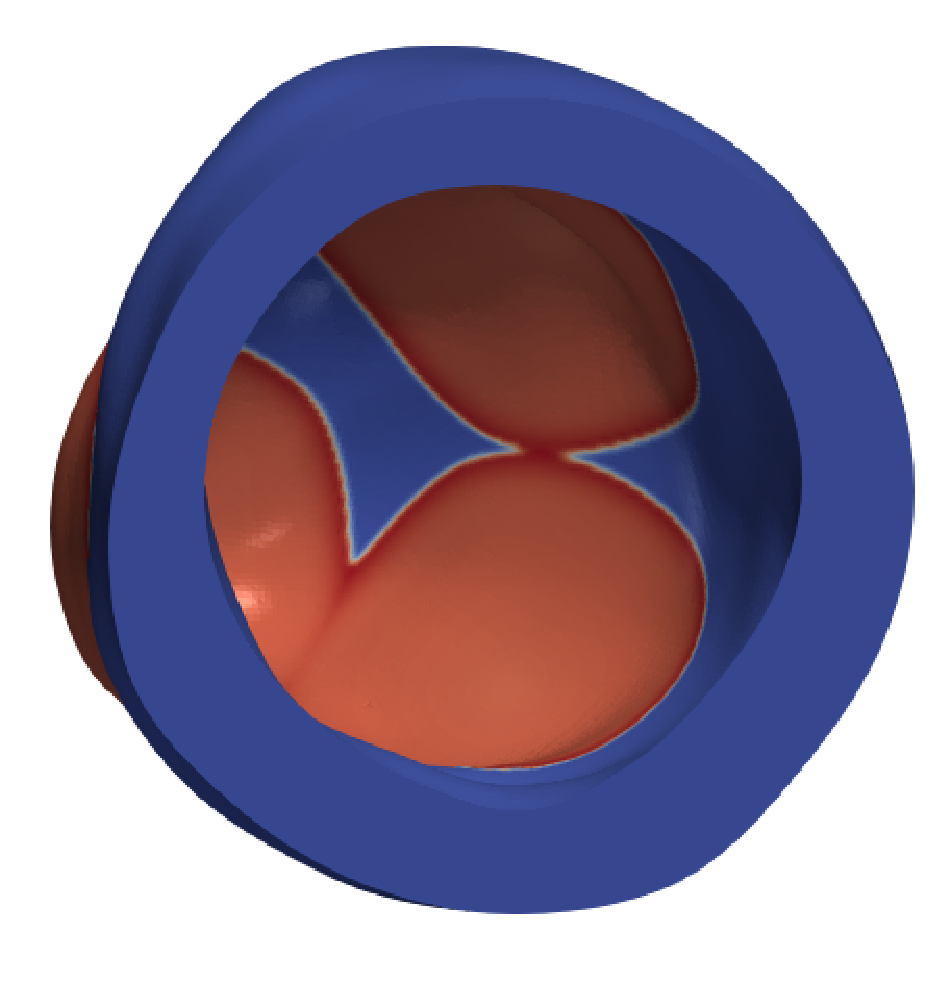
\includegraphics[width=\linewidth]{fig/view_impulses.pdf}
        \caption{}
        \label{subfig:left_ventricle_impulses}
    \end{subfigure}

    \caption{
        (\subref{subfig:left_ventricle_mesh}) Hexahedral mesh representing a realistic left ventricle.
        (\subref{subfig:left_ventricle_impulses}) Propagation of the transmembrane potential.
    }
    \label{fig:left_ventricle}
\end{figure}

\begin{figure}[h!]
    \centering
    \includegraphics[width=0.9\textwidth]{fig/iterates_3D_monodomain.pdf}
    \caption{Number of preconditioned conjugate-gradient (PCG) iterations per time step for the monodomain problem, comparing AMG and agglomerated multigrid (AggloMG) for polynomial degrees $p\!=\!1,2$ for the three-dimensional
        ventricle test.}
    \label{fig:iterates_3D_monodomain}
\end{figure}


\begin{figure}[h!]
    \centering
    \includegraphics[width=0.9\textwidth]{fig/iteration_times_3D_monodomain.pdf}
    \caption{PCG iteration time per time step for the monodomain problem, comparing AMG and agglomerated multigrid (AggloMG) for polynomial degrees $p\!=\!1,2$ for the three-dimensional
        ventricle test. Results have been obtained on 128 MPI processes on the Toeplitz cluster at University of Pisa.}
    \label{fig:iteration_times_3D_monodomain}
\end{figure}










\newpage

\section{{Integration of PSCToolkit}}
\label{sec:section5}



\subsection{{[Subsection Title]}}



\newpage

\section{{Integration of MUMPS}}
\label{sec:section6}


\newpage

\section{{Conclusion}} \label{sec:conclusion}

\begin{thebibliography}{10}
    \bibitem[Cangiani et al., 2014]{polyDG}Andrea Cangiani, Emmanuil Georgoulis and Paul Houston, "hp-Version discontinuous Galerkin methods on polygonal and polyhedral meshes," Mathematical Models and Methods in Applied Sciences, vol. 24, no. 4, pp. 2009-2041, 2014.
    \bibitem[Antonietti et al., 2013]{Antoniettihp}Paola Antonietti, Stefano Giani, and Paul Houston, "$hp$-Version Composite Discontinuous Galerkin Methods for Elliptic Problems on Complicated Domains", SIAM Journal on Scientific Computing, vol. 35, A1417-A1439, 2013.
    \bibitem[Feder et al., 2025]{FEDER2025113773}Marco Feder, Andrea Cangiani and Luca Heltai, "R3MG: R-tree based agglomeration of polytopal grids with applications to multilevel methods", Journal of Computational Physics, vol. 526, 113773, 2025.
    \bibitem[Feder and Africa, 2026]{feder2026agglomeration}Marco Feder and Pasquale Claudio Africa, "An agglomeration-based multigrid solver for the discontinuous Galerkin discretization of cardiac electrophysiology", arXiv preprint arXiv:2602.16312, 2026.
    \bibitem[Kronbichler and Kormann, 2019]{KronbichlerKormann}Martin Kronbichler and Katharina Kormann, "Fast Matrix-Free Evaluation of Discontinuous Galerkin Finite Element Operators", ACM Transactions on Mathematical Software, vol. 45, no. 3, Article 29, 2019.

\end{thebibliography}



\label{MyLastPage}

\end{document}
